% -*- mode: Noweb; noweb-code-mode: perl-mode; tab-width: 4 -*-% ===> this file was generated automatically by noweave --- better not edit it
\documentclass[11pt]{article}
%
%2345678901234567890123456789012345678901234567890123456789012345678901234567890
%        1         2         3         4         5         6         7         8
%
% $Id: SintenicGenePrediction.tex,v 1.1.1.1 2001-06-02 11:24:16 jabril Exp $
%
\usepackage{noweb}
\usepackage[a4paper,offset={0pt,0pt},hmargin={2cm,2cm},vmargin={1cm,1cm}]{geometry}
\usepackage{graphics}
\usepackage[dvips]{graphicx}
%% pstricks
\usepackage[dvips]{pstcol}
\usepackage{pstricks}
%\usepackage{pst-node}
%\usepackage{pst-char}
%\usepackage{pst-grad}
%% bibliography
\usepackage{natbib}
%% latex2html
\usepackage{url}
\usepackage{html}     
\usepackage{htmllist} 
%% tables    
%\usepackage{colortbl}
%\usepackage{multirow}
%\usepackage{hhline}
%\usepackage{tabularx}
%\usepackage{dcolumn}
%% seminar
%\usepackage{semcolor,semlayer,semrot,semhelv,sem-page,slidesec}
%% draft watermark
%\usepackage[all,dvips]{draftcopy}
%\draftcopySetGrey{0.9}
%\draftcopyName{CONFIDENTIAL}{100}
%% layout
\usepackage{fancyhdr} % Do not use \usepackage{fancybox} -> TOCs disappear
%\usepackage{lscape}
%\usepackage{rotating}
%\usepackage{multicol}
%% fonts
\usepackage{times}\fontfamily{ptm}\selectfont
\usepackage{t1enc}

% noweb options
\noweboptions{smallcode}
\def\nwendcode{\endtrivlist \endgroup} % relax page breaking scheme
\let\nwdocspar=\par                    %
 
% Colors for gff2ps
\input ColorDefs.tex
% New Commands are defined here
\newcommand{\sctn}[1]{\section{#1}}
\newcommand{\subsctn}[1]{\subsection{#1}}
\newcommand{\subsubsctn}[1]{\subsubsection{#1}}
\newcommand{\desc}[1]{\item[#1] \ \\}

% PSTRICKs definitions
\pslongbox{ExFrame}{\psframebox}
\newcommand{\cln}[1]{\fcolorbox{black}{#1}{\textcolor{#1}{\rule[-.3ex]{1cm}{1ex}}}}
\newpsobject{showgrid}{psgrid}{subgriddiv=0,griddots=1,gridlabels=6pt}
% \pscharpath[fillstyle=solid, fillcolor=verydarkcyan, linecolor=black, linewidth=1pt]{\sffamily\scshape\bfseries\veryHuge #1 }

%%%%% global urls
% \newcommand{\getpsf}[1]{\html{(\htmladdnormallink{Get PostScript file}{./Psfiles/#1})}}   
\def\mtjabril{\htmladdnormallink{\textbf{jabril@imim.es}}{MAILTO:jabril@imim.es}}

% defs
\def\drome{\textit{Drosophila melanogaster}}
\def\dro{\textit{Drosophila}}
\def\dme{\textit{D. melanogaster}}
\def\seq{\texttt{\textbf{X62937}}}
\def\nowf{{\Tt{}SintenicGenePrediction.nw}}
\def\rptm{\textsc{RepeatMasker}}
\def\bl{\textsc{Blast}}
\def\bn{\textsc{blastn}}
\def\bx{\textsc{blastx}}
\def\bp{\textsc{blastp}}
\def\tbn{\textsc{tblastn}}
\def\tbx{\textsc{tblastx}}
\def\ps{\textsc{PostScript}}
\def\gnid{\texttt{geneid}}
\def\gnsc{\texttt{genscan}}
\def\prog{\textsc{sgp}}

% Setting text for footers and headers

\def\tit{\textsc{Sintenic Gene Prediction Tool.- }}
\fancyhead{} % clear all fields
\fancyfoot{} % clear all fields
\fancyhead[RO,LE]{\thepage}
\fancyhead[LO,RE]{\rightmark}
\fancyfoot[LO,LE]{\small\textsl{Guig\`o, Parra, Abril}}
\fancyfoot[RO,RE]{\small\textbf{\today}}
\renewcommand{\headrulewidth}{1pt}
\renewcommand{\footrulewidth}{1pt}

%%%%%%%%%%%%%%%%%%%%%%%%%%%%%%%%%%%%%%%%%%%%%%%%%%%%%%%%%%%%%%%%%%%%%%%%%%%

\begin{document}
\nwfilename{/home/ug/jabril/development/sggp/SintenicGenePrediction.nw}\nwbegindocs{1}\nwdocspar
\thispagestyle{empty}

\begin{titlepage}

\ \vfill
\begin{center}
\textbf{\Huge Sintenic Gene Prediction Tool}\\[5ex]

\textbf{\Large Roderic Guig\`o}\\[1ex]
\textbf{\Large Gen\'{\i}s Parra}\\[1ex]
\textbf{\Large Josep F. Abril}\\[5ex] % \raisebox{0.85ex}{\footnotesize$\,\dag$}\\[0.5ex]

\textbf{\large --- \today ---}\\[10ex]

\begin{abstract}
\begin{center}
\parbox{0.75\linewidth}{
The project main goal is to implement the {\prog} tool in Perl, make its parameters able to get configured through a customization file, and draft a script to automatize fine tunning of the program. We have to include in the distributable package a modified version of {\gnid}. We will need to optimize the {\bl} databases in order to increase query search speed when long subject sequences are given.
} % parbox
\end{center}
\end{abstract}

\vfill

\begin{raggedleft}
\scalebox{0.9 1}{\Large\textsl{\textbf{Genome Informatics Research Lab}}}\\
Grup de Recerca en Infom\`atica Biom\`edica\\
Institut Municipal d'Investigaci\'o M\`edica\\
Universitat Pompeu Fabra\\[2ex]
\raisebox{0.85ex}{\footnotesize$\dag\,$}{\large e-mail: \mtjabril}\\
\end{raggedleft}
\end{center}

\end{titlepage} %'

%%%%%%%%%%%%%%%%%%%% FRONTMATTER

\newpage
\pagenumbering{roman}
\setcounter{page}{1}
\pagestyle{fancy}
% Marks redefinition must go here because pagestyle 
% resets the values to the default ones.
\renewcommand{\sectionmark}[1]{\markboth{}{\thesection.\ #1}}
\renewcommand{\subsectionmark}[1]{\markboth{}{\thesubsection.\ \textsl{#1}}}

\tableofcontents
\listoftables
\listoffigures

\vfill
\begin{center}
{\small$<$ \verb$Id: SintenicGenePrediction.tex,v 1.1.1.1 2001-06-02 11:24:16 jabril Exp $$>$ }
\end{center}

%%%%%%%%%%%%%%%%%%%% MAINMATTER

\newpage
\pagenumbering{arabic}
\setcounter{page}{1}

\sctn{Introduction}

\subsctn{On using comparative genomics to improve gene prediction at genomic scale.}

Conservation in the genomic sequence of species at the appropiate
phylogenetic distance may be indicative of conservation of sequence
function.  We investigate here how sequence conservation may be
indicative of coding function, and develop program, SGP-2, which
integrates the results from {\gnid} and {\tbx} to produce gene
predictions when comparing human/mouse sintenic regions.  We set up a
number benchmark data sets, in which we benchmark {\prog} efficiency
and we test it against \textit{ab initio} programs, sequence similarity
based programs, and other hibrid programs.

% How the program works...
\subsctn{Overall algorithm}

Figure~\ref{fig:algo2} describes the approach in {\prog}.  Given two
genomic sequences, we follow the protocol outlined here: 

\begin{enumerate}
\item mask the sequences using {\rptm},
\item run {\tbx} of one sequence agains the other,
\item ``project'' the similarity regions onto each sequence,
\item  run {\gnid} on each sequence with the projected similarity regions.
\end{enumerate}

\begin{figure}
\begin{center}
\framebox{
\includegraphics[width=0.85\linewidth, trim= 10 10 20 10, clip]{./psfigures/algo2.ps}
}
\end{center}
\caption{\label{fig:algo2} Schemma of the homology-based gene-prediction used in this project.}
\end{figure}

\sctn{The parameters file}

\sctn{Parameter optimization}

%%%%%%%%%%%%%%%%%%%%%%%%%%%%%%%%%%%
\begin{comment}
\end{comment}
%%%%%%%%%%%%%%%%%%%%%%%%%%%%%%%%%%%

%%%%%%%%%%%%%%%%%%%% BACKMATTER

% \newpage
% 
% \bibliographystyle{apalike}
% \bibliography{/home1/rguigo/docs/biblio/References}

\newpage
\appendix

\sctn{Sintenic Gene Prediction tool}

Our initial program outline (our root chunk) looks like:\\[1ex]

\nwenddocs{}\nwbegincode{2}\sublabel{NWSinw-SGP8-1}\nwmargintag{{\nwtagstyle{}\subpageref{NWSinw-SGP8-1}}}\moddef{SGP TOOL~{\nwtagstyle{}\subpageref{NWSinw-SGP8-1}}}\endmoddef\nwstartdeflinemarkup\nwenddeflinemarkup
\LA{}PERL shebang~{\nwtagstyle{}\subpageref{NWSinw-PERC-1}}\RA{}
\LA{}SGP Copyleft~{\nwtagstyle{}\subpageref{NWSinw-SGPC-1}}\RA{}

#### CONSTANTS DEFINITION ####


#### VARIABLES DECLARATION ####


#### MAIN LOOP ####

  \LA{}Main Loop - SGP~{\nwtagstyle{}\subpageref{nw@notdef}}\RA{}

##### SUBS #####

\LA{}SGP: parsing command-line~{\nwtagstyle{}\subpageref{NWSinw-SGPP-1}}\RA{}
\LA{}SGP: parsing parameters file~{\nwtagstyle{}\subpageref{NWSinw-SGPS-1}}\RA{}
\LA{}SGP: run blast~{\nwtagstyle{}\subpageref{NWSinw-SGPE-1}}\RA{}
\LA{}SGP: extract HSPs~{\nwtagstyle{}\subpageref{NWSinw-SGPH-1}}\RA{}
\LA{}SGP: run geneid~{\nwtagstyle{}\subpageref{NWSinw-SGPF-1}}\RA{}
\LA{}SGP: graphical output~{\nwtagstyle{}\subpageref{NWSinw-SGPL-1}}\RA{}

#### EOF ####

\LA{}POD man page - SGP~{\nwtagstyle{}\subpageref{NWSinw-PODI-1}}\RA{}
\nwnotused{SGP TOOL}\nwendcode{}\nwbegindocs{3}% 

A short description, followed by authors list and the GNU-GPL is described here.

\nwenddocs{}\nwbegincode{4}\sublabel{NWSinw-SGPC-1}\nwmargintag{{\nwtagstyle{}\subpageref{NWSinw-SGPC-1}}}\moddef{SGP Copyleft~{\nwtagstyle{}\subpageref{NWSinw-SGPC-1}}}\endmoddef\nwstartdeflinemarkup\nwusesondefline{\\{NWSinw-SGP8-1}}\nwenddeflinemarkup
######################################################################
#                               SGP                                  #
######################################################################
#
#     Sinteny based Gene Prediction tool.
#
#     Copyright (C) 2000 - Josep Francesc ABRIL FERRANDO
#                                   Genis PARRA FARRE
#                                 Roderic GUIGO SERRA
\LA{}Copyleft~{\nwtagstyle{}\subpageref{NWSinw-Cop8-1}}\RA{}
\nwused{\\{NWSinw-SGP8-1}}\nwendcode{}\nwbegindocs{5}\nwdocspar

\subsctn{Parsing command-line options}

\nwenddocs{}\nwbegincode{6}\sublabel{NWSinw-SGPP-1}\nwmargintag{{\nwtagstyle{}\subpageref{NWSinw-SGPP-1}}}\moddef{SGP: parsing command-line~{\nwtagstyle{}\subpageref{NWSinw-SGPP-1}}}\endmoddef\nwstartdeflinemarkup\nwusesondefline{\\{NWSinw-SGP8-1}}\nwenddeflinemarkup
\nwused{\\{NWSinw-SGP8-1}}\nwendcode{}\nwbegindocs{7}% 

\subsctn{Parsing parameters file}

\nwenddocs{}\nwbegincode{8}\sublabel{NWSinw-SGPS-1}\nwmargintag{{\nwtagstyle{}\subpageref{NWSinw-SGPS-1}}}\moddef{SGP: parsing parameters file~{\nwtagstyle{}\subpageref{NWSinw-SGPS-1}}}\endmoddef\nwstartdeflinemarkup\nwusesondefline{\\{NWSinw-SGP8-1}}\nwenddeflinemarkup
\nwused{\\{NWSinw-SGP8-1}}\nwendcode{}\nwbegindocs{9}%

\subsctn{Running {\bl} on sequences}

\nwenddocs{}\nwbegincode{10}\sublabel{NWSinw-SGPE-1}\nwmargintag{{\nwtagstyle{}\subpageref{NWSinw-SGPE-1}}}\moddef{SGP: run blast~{\nwtagstyle{}\subpageref{NWSinw-SGPE-1}}}\endmoddef\nwstartdeflinemarkup\nwusesondefline{\\{NWSinw-SGP8-1}}\nwenddeflinemarkup
\nwused{\\{NWSinw-SGP8-1}}\nwendcode{}\nwbegindocs{11}% 

\subsctn{Processing HSPs from {\bl}}

\nwenddocs{}\nwbegincode{12}\sublabel{NWSinw-SGPH-1}\nwmargintag{{\nwtagstyle{}\subpageref{NWSinw-SGPH-1}}}\moddef{SGP: extract HSPs~{\nwtagstyle{}\subpageref{NWSinw-SGPH-1}}}\endmoddef\nwstartdeflinemarkup\nwusesondefline{\\{NWSinw-SGP8-1}}\nwenddeflinemarkup
\nwused{\\{NWSinw-SGP8-1}}\nwendcode{}\nwbegindocs{13}% 

\subsctn{Running {\gnid} on SRs}

\nwenddocs{}\nwbegincode{14}\sublabel{NWSinw-SGPF-1}\nwmargintag{{\nwtagstyle{}\subpageref{NWSinw-SGPF-1}}}\moddef{SGP: run geneid~{\nwtagstyle{}\subpageref{NWSinw-SGPF-1}}}\endmoddef\nwstartdeflinemarkup\nwusesondefline{\\{NWSinw-SGP8-1}}\nwenddeflinemarkup
\nwused{\\{NWSinw-SGP8-1}}\nwendcode{}\nwbegindocs{15}% 

\subsctn{Making plots}

\nwenddocs{}\nwbegincode{16}\sublabel{NWSinw-SGPL-1}\nwmargintag{{\nwtagstyle{}\subpageref{NWSinw-SGPL-1}}}\moddef{SGP: graphical output~{\nwtagstyle{}\subpageref{NWSinw-SGPL-1}}}\endmoddef\nwstartdeflinemarkup\nwusesondefline{\\{NWSinw-SGP8-1}}\nwenddeflinemarkup
\nwused{\\{NWSinw-SGP8-1}}\nwendcode{}\nwbegindocs{17}% 

%%%%%%%%%%%%%%%%%%%%%%%%%%%%%%%%%%%
\begin{comment}
\end{comment}
%%%%%%%%%%%%%%%%%%%%%%%%%%%%%%%%%%%

\newpage

\sctn{License Terms}

The programs are distributed under GNU General Public License as described below.  Those are the license terms that must appear at programs begining.

\nwenddocs{}\nwbegincode{18}\sublabel{NWSinw-Cop8-1}\nwmargintag{{\nwtagstyle{}\subpageref{NWSinw-Cop8-1}}}\moddef{Copyleft~{\nwtagstyle{}\subpageref{NWSinw-Cop8-1}}}\endmoddef\nwstartdeflinemarkup\nwusesondefline{\\{NWSinw-SGPC-1}}\nwenddeflinemarkup
#
# This program is free software; you can redistribute it and/or modify
# it under the terms of the GNU General Public License as published by
# the Free Software Foundation; either version 2 of the License, or
# (at your option) any later version.
#
# This program is distributed in the hope that it will be useful,
# but WITHOUT ANY WARRANTY; without even the implied warranty of
# MERCHANTABILITY or FITNESS FOR A PARTICULAR PURPOSE.  See the
# GNU General Public License for more details.
#
# You should have received a copy of the GNU General Public License
# along with this program; if not, write to the Free Software
# Foundation, Inc., 675 Mass Ave, Cambridge, MA 02139, USA.
#
######################################################################
#
\nwused{\\{NWSinw-SGPC-1}}\nwendcode{}\nwbegindocs{19}\nwdocspar

\newpage

\sctn{POD Pages}

The documentation for {\Tt{}perl} programs is written in a simple markup language called POD (Plain Old Documentation). Translators exist for {\Tt{}pod2man}, {\Tt{}pod2text}, {\Tt{}pod2html}, {\Tt{}pod2latex}, and {\Tt{}pod2fm}. 
The idea is to have the online documentation included with the source. That is possible with {\Tt{}{\_}{\_}DATA{\_}{\_}} tag, which defines a chunk of data within the same file.
%% TODO: define POD tags and which style was used for building up this man. 

\nwenddocs{}\nwbegincode{20}\sublabel{NWSinw-PODI-1}\nwmargintag{{\nwtagstyle{}\subpageref{NWSinw-PODI-1}}}\moddef{POD man page - SGP~{\nwtagstyle{}\subpageref{NWSinw-PODI-1}}}\endmoddef\nwstartdeflinemarkup\nwusesondefline{\\{NWSinw-SGP8-1}}\nwenddeflinemarkup
__DATA__

=head1 NAME

    
$PROGRAM ($VERSION) - Improving Gene Prediction with Sinteny.

=head1 SYNOPSIS

    
    $PROGRAM [-hv] [-o 'options'] [-g 'options'] \\
      [-P filename] [-p filename] [-k filename] \\
      [-c value] [-s value] -1 seqfile_1 -2 seqfile_2

=head1 DESCRIPTION

=head1 OPTIONS

    

=over 4

=item B<-1> I<seqfile_1>

input file for first species.

=item B<-2> I<seqfile_2>

input file for second species.

=item B<-g>

geneid options

=item B<-o>

tblastx options

=item B<-c> I<value>

tblastx score cuttof

=item B<-s> I<value>

shrink hsp\\'s by value

=item B<-t> I<filename>

read tblastx file

=item B<-f> I<prefix>

read hsp gff files with in directory prefix and extension .hsp-rs

=item B<-k> I<prefix>

keep intermediate files with prefix

=item B<-p> I<filename>

ps output in filename file 

=item B<-P> I<filename>

geneid parameter file

=item B<-v>

verbose mode

=item B<-h>

produces this message

=back

=head1 FILES

=head1 DIAGNOSTICS

=head1 REQUIRES

=head1 BUGS

    
Report any problem to: B<jabril@imim.es>

=head1 AUTHOR

    
Roderic Guigo   : B<rguigo@imim.es>

Josep F. Abril  : B<jabril@imim.es>

Genis Parra     : B<gparra@imim.es>

B<$PROGRAM> is under GNU-GPL (C) 2000
\nwused{\\{NWSinw-SGP8-1}}\nwendcode{}\nwbegindocs{21}%$

\newpage

\sctn{Common code blocks}

\subsctn{PERL scripts}

\nwenddocs{}\nwbegincode{22}\sublabel{NWSinw-PERC-1}\nwmargintag{{\nwtagstyle{}\subpageref{NWSinw-PERC-1}}}\moddef{PERL shebang~{\nwtagstyle{}\subpageref{NWSinw-PERC-1}}}\endmoddef\nwstartdeflinemarkup\nwusesondefline{\\{NWSinw-SGP8-1}}\nwenddeflinemarkup
#!/usr/bin/perl -w
# This is perl, version 5.005_03 built for i386-linux
#
\LA{}Version Control Id Tag~{\nwtagstyle{}\subpageref{NWSinw-VerM-1}}\RA{}
#
use strict;
#
\nwused{\\{NWSinw-SGP8-1}}\nwendcode{}\nwbegindocs{23}\nwdocspar

\nwenddocs{}\nwbegincode{24}\sublabel{NWSinw-GloQ-1}\nwmargintag{{\nwtagstyle{}\subpageref{NWSinw-GloQ-1}}}\moddef{Global Constants - Boolean~{\nwtagstyle{}\subpageref{NWSinw-GloQ-1}}}\endmoddef\nwstartdeflinemarkup\nwenddeflinemarkup
my ($T,$F) = (1,0); # for 'T'rue and 'F'alse
\nwindexdefn{\nwixident{{\$}T}}{:doT}{NWSinw-GloQ-1}\nwindexdefn{\nwixident{{\$}F}}{:doF}{NWSinw-GloQ-1}\eatline
\nwnotused{Global Constants - Boolean}\nwidentdefs{\\{{\nwixident{{\$}F}}{:doF}}\\{{\nwixident{{\$}T}}{:doT}}}\nwendcode{}\nwbegindocs{25}\nwdocspar
We also set here the date when the script is running and who is the user running it.

\nwenddocs{}\nwbegincode{26}\sublabel{NWSinw-GloR-1}\nwmargintag{{\nwtagstyle{}\subpageref{NWSinw-GloR-1}}}\moddef{Global Vars - User and Date~{\nwtagstyle{}\subpageref{NWSinw-GloR-1}}}\endmoddef\nwstartdeflinemarkup\nwenddeflinemarkup
my $DATE = localtime;
my $USER = $ENV\{USER\};
\nwindexdefn{\nwixident{{\$}DATE}}{:doDATE}{NWSinw-GloR-1}\nwindexdefn{\nwixident{{\$}USER}}{:doUSER}{NWSinw-GloR-1}\eatline
\nwnotused{Global Vars - User and Date}\nwidentdefs{\\{{\nwixident{{\$}DATE}}{:doDATE}}\\{{\nwixident{{\$}USER}}{:doUSER}}}\nwendcode{}\nwbegindocs{27}\nwdocspar

\subsubsctn{Timing our scripts}

The '{\Tt{}Benchmark}' module encapsulates a number of routines to help to figure out how long it takes to execute a piece of code and the whole script.

\nwenddocs{}\nwbegincode{28}\sublabel{NWSinw-UseN-1}\nwmargintag{{\nwtagstyle{}\subpageref{NWSinw-UseN-1}}}\moddef{Use Modules - Benchmark~{\nwtagstyle{}\subpageref{NWSinw-UseN-1}}}\endmoddef\nwstartdeflinemarkup\nwenddeflinemarkup
use Benchmark;
  \LA{}Timer ON~{\nwtagstyle{}\subpageref{NWSinw-Tim8-1}}\RA{}
\nwnotused{Use Modules - Benchmark}\nwendcode{}\nwbegindocs{29}\nwdocspar

See '{\Tt{}man\ Benchmark}' for further info about this package. 
We set an array to keep record of timing for each section.

\nwenddocs{}\nwbegincode{30}\sublabel{NWSinw-Tim8-1}\nwmargintag{{\nwtagstyle{}\subpageref{NWSinw-Tim8-1}}}\moddef{Timer ON~{\nwtagstyle{}\subpageref{NWSinw-Tim8-1}}}\endmoddef\nwstartdeflinemarkup\nwusesondefline{\\{NWSinw-UseN-1}}\nwenddeflinemarkup
my @Timer = (new Benchmark);
\nwused{\\{NWSinw-UseN-1}}\nwendcode{}\nwbegindocs{31}\nwdocspar

\nwenddocs{}\nwbegincode{32}\sublabel{NWSinw-ComS-1}\nwmargintag{{\nwtagstyle{}\subpageref{NWSinw-ComS-1}}}\moddef{Common PERL subs - Benchmark~{\nwtagstyle{}\subpageref{NWSinw-ComS-1}}}\endmoddef\nwstartdeflinemarkup\nwenddeflinemarkup
sub timing() \{
    push @Timer, (new Benchmark);
    # partial time 
    $_[0] || 
        (return timestr(timediff($Timer[$#Timer],$Timer[($#Timer - 1)])));
    # total time
    return timestr(timediff($Timer[$#Timer],$Timer[0]));
\} # timing
\nwnotused{Common PERL subs - Benchmark}\nwendcode{}\nwbegindocs{33}\nwdocspar


\subsubsctn{Printing complex Data Structures}

With '{\Tt{}Data::Dumper}' we are able to pretty print complex data structures for debugging them.


\nwenddocs{}\nwbegincode{34}\sublabel{NWSinw-UseK-1}\nwmargintag{{\nwtagstyle{}\subpageref{NWSinw-UseK-1}}}\moddef{Use Modules - Dumper~{\nwtagstyle{}\subpageref{NWSinw-UseK-1}}}\endmoddef\nwstartdeflinemarkup\nwenddeflinemarkup
use Data::Dumper;
local $Data::Dumper::Purity = 0;
local $Data::Dumper::Deepcopy = 1;
\nwnotused{Use Modules - Dumper}\nwendcode{}\nwbegindocs{35}\nwdocspar


\subsubsctn{Common functions}

\nwenddocs{}\nwbegincode{36}\sublabel{NWSinw-SkiV-1}\nwmargintag{{\nwtagstyle{}\subpageref{NWSinw-SkiV-1}}}\moddef{Skip comments and empty records~{\nwtagstyle{}\subpageref{NWSinw-SkiV-1}}}\endmoddef\nwstartdeflinemarkup\nwenddeflinemarkup
next if /^\\#/o;
next if /^\\s*$/o;
chomp;
\nwnotused{Skip comments and empty records}\nwendcode{}\nwbegindocs{37}\nwdocspar

\nwenddocs{}\nwbegincode{38}\sublabel{NWSinw-ComQ-1}\nwmargintag{{\nwtagstyle{}\subpageref{NWSinw-ComQ-1}}}\moddef{Common PERL subs - Min Max~{\nwtagstyle{}\subpageref{NWSinw-ComQ-1}}}\endmoddef\nwstartdeflinemarkup\nwenddeflinemarkup
#
sub max() \{
    my $z = shift @_;
    foreach my $l (@_) \{ $z = $l if $l > $z \};
    return $z;
\} # max
sub min() \{
    my $z = shift @_;
    foreach my $l (@_) \{ $z = $l if $l < $z \};
    return $z;
\} # min
\nwnotused{Common PERL subs - Min Max}\nwendcode{}\nwbegindocs{39}\nwdocspar

\nwenddocs{}\nwbegincode{40}\sublabel{NWSinw-ComS.2-1}\nwmargintag{{\nwtagstyle{}\subpageref{NWSinw-ComS.2-1}}}\moddef{Common PERL subs - Text fill~{\nwtagstyle{}\subpageref{NWSinw-ComS.2-1}}}\endmoddef\nwstartdeflinemarkup\nwenddeflinemarkup
#
sub fill_right() \{ $_[0].($_[2] x ($_[1] - length($_[0]))) \}
sub fill_left()  \{ ($_[2] x ($_[1] - length($_[0]))).$_[0] \}
sub fill_mid()   \{ 
    my $l = length($_[0]);
    my $k = int(($_[1] - $l)/2);
    ($_[2] x $k).$_[0].($_[2] x ($_[1] - ($l+$k)));
\} # fill_mid
\nwnotused{Common PERL subs - Text fill}\nwendcode{}\nwbegindocs{41}\nwdocspar

These functions are used to report to STDERR a single char for each record processed (useful for reporting parsed records).

\nwenddocs{}\nwbegincode{42}\sublabel{NWSinw-ComQ.2-1}\nwmargintag{{\nwtagstyle{}\subpageref{NWSinw-ComQ.2-1}}}\moddef{Common PERL subs - Counter~{\nwtagstyle{}\subpageref{NWSinw-ComQ.2-1}}}\endmoddef\nwstartdeflinemarkup\nwenddeflinemarkup
#
sub counter \{ # $_[0]~current_pos++ $_[1]~char
    print STDERR "$_[1]";
    (($_[0] % 50) == 0) && (print STDERR "[".&fill_left($_[0],6,"0")."]\\n");
\} # counter
#
sub counter_end \{ # $_[0]~current_pos   $_[1]~char
    (($_[0] % 50) != 0) && (print STDERR "[".&fill_left($_[0],6,"0")."]\\n");
\} # counter_end
\nwnotused{Common PERL subs - Counter}\nwendcode{}\nwbegindocs{43}\nwdocspar

\nwenddocs{}\nwbegincode{44}\sublabel{NWSinw-GloL-1}\nwmargintag{{\nwtagstyle{}\subpageref{NWSinw-GloL-1}}}\moddef{Global Vars - Counter~{\nwtagstyle{}\subpageref{NWSinw-GloL-1}}}\endmoddef\nwstartdeflinemarkup\nwenddeflinemarkup
my ($n,$c); # counter and char (for &counter function)
\nwindexdefn{\nwixident{{\$}n}}{:don}{NWSinw-GloL-1}\nwindexdefn{\nwixident{{\$}c}}{:doc}{NWSinw-GloL-1}\eatline
\nwnotused{Global Vars - Counter}\nwidentdefs{\\{{\nwixident{{\$}c}}{:doc}}\\{{\nwixident{{\$}n}}{:don}}}\nwendcode{}\nwbegindocs{45}\nwdocspar

\subsubsctn{Common functions for reporting program processes}
\label{sec:messagerpt}

Function '{\Tt{}report}' requires that a hash variable '{\Tt{}{\%}MessageList}' has been set, such hash contains the strings for each report message we will need. The first parameter for '{\Tt{}report}' is a key for that hash, in order to retrieve the message string, the other parameters passed are processed by the {\Tt{}sprintf} function on that string.

\nwenddocs{}\nwbegincode{46}\sublabel{NWSinw-ComP-1}\nwmargintag{{\nwtagstyle{}\subpageref{NWSinw-ComP-1}}}\moddef{Common PERL subs - STDERR~{\nwtagstyle{}\subpageref{NWSinw-ComP-1}}}\endmoddef\nwstartdeflinemarkup\nwprevnextdefs{\relax}{NWSinw-ComP-2}\nwenddeflinemarkup
sub report() \{ print STDERR sprintf($MessageList\{ shift @_ \},@_) \}
\nwalsodefined{\\{NWSinw-ComP-2}}\nwnotused{Common PERL subs - STDERR}\nwendcode{}\nwbegindocs{47}\nwdocspar

The same happens to '{\Tt{}warn}' function which also requires a hash variable '{\Tt{}{\%}ErrorList}' containing the error messages.

\nwenddocs{}\nwbegincode{48}\sublabel{NWSinw-ComP-2}\nwmargintag{{\nwtagstyle{}\subpageref{NWSinw-ComP-2}}}\moddef{Common PERL subs - STDERR~{\nwtagstyle{}\subpageref{NWSinw-ComP-1}}}\plusendmoddef\nwstartdeflinemarkup\nwprevnextdefs{NWSinw-ComP-1}{\relax}\nwenddeflinemarkup
sub warn() \{ print STDERR sprintf($ErrorList\{ shift @_ \}, @_) \}
\nwendcode{}\nwbegindocs{49}\nwdocspar

\subsctn{AWK scripts}

\nwenddocs{}\nwbegincode{50}\sublabel{NWSinw-GAWC-1}\nwmargintag{{\nwtagstyle{}\subpageref{NWSinw-GAWC-1}}}\moddef{GAWK shebang~{\nwtagstyle{}\subpageref{NWSinw-GAWC-1}}}\endmoddef\nwstartdeflinemarkup\nwenddeflinemarkup
#!/usr/bin/gawk -f
# GNU Awk 3.0.4
\LA{}Version Control Id Tag~{\nwtagstyle{}\subpageref{NWSinw-VerM-1}}\RA{}
\nwnotused{GAWK shebang}\nwendcode{}\nwbegindocs{51}\nwdocspar

\subsctn{BASH scripts}

\nwenddocs{}\nwbegincode{52}\sublabel{NWSinw-BASC-1}\nwmargintag{{\nwtagstyle{}\subpageref{NWSinw-BASC-1}}}\moddef{BASH shebang~{\nwtagstyle{}\subpageref{NWSinw-BASC-1}}}\endmoddef\nwstartdeflinemarkup\nwusesondefline{\\{NWSinw-wea7-1}\\{NWSinw-LaT8-1}}\nwenddeflinemarkup
#!/usr/bin/bash
# GNU bash, version 2.03.6(1)-release (i386-redhat-linux-gnu)
\LA{}Version Control Id Tag~{\nwtagstyle{}\subpageref{NWSinw-VerM-1}}\RA{}
#
SECONDS=0 # Reset Timing
# Which script are we running...
L="####################"
\{ echo "$L$L$L$L";
  echo "### RUNNING [$0]";
  echo "### Current date:`date`";
  echo "###"; \} 1>&2;
\nwused{\\{NWSinw-wea7-1}\\{NWSinw-LaT8-1}}\nwendcode{}\nwbegindocs{53}\nwdocspar

\nwenddocs{}\nwbegincode{54}\sublabel{NWSinw-BASF-1}\nwmargintag{{\nwtagstyle{}\subpageref{NWSinw-BASF-1}}}\moddef{BASH script end~{\nwtagstyle{}\subpageref{NWSinw-BASF-1}}}\endmoddef\nwstartdeflinemarkup\nwusesondefline{\\{NWSinw-wea7-1}\\{NWSinw-LaT8-1}}\nwenddeflinemarkup
\{ echo "###"; echo "### Execution time for [$0] : $SECONDS secs";
  echo "$L$L$L$L";
  echo ""; \} 1>&2;
#
exit 0
\nwused{\\{NWSinw-wea7-1}\\{NWSinw-LaT8-1}}\nwendcode{}\nwbegindocs{55}\nwdocspar

\subsctn{Version control tags}

This document is under Revision Control System (RCS). The version you are currently reading is the following:

\nwenddocs{}\nwbegincode{56}\sublabel{NWSinw-VerM-1}\nwmargintag{{\nwtagstyle{}\subpageref{NWSinw-VerM-1}}}\moddef{Version Control Id Tag~{\nwtagstyle{}\subpageref{NWSinw-VerM-1}}}\endmoddef\nwstartdeflinemarkup\nwusesondefline{\\{NWSinw-PERC-1}\\{NWSinw-GAWC-1}\\{NWSinw-BASC-1}}\nwenddeflinemarkup
# $Id: SintenicGenePrediction.tex,v 1.1.1.1 2001-06-02 11:24:16 jabril Exp $
\nwused{\\{NWSinw-PERC-1}\\{NWSinw-GAWC-1}\\{NWSinw-BASC-1}}\nwendcode{}\nwbegindocs{57}\nwdocspar

\newpage

\sctn{Extracting code blocks from this document}

From this file we can obtain both the code and the
documentation. The following instructions are needed:

\subsctn{Extracts Script code chunks from the {\Tt{}noweb} file} % \\[-0.5ex]

Remember when tangling that '-L' option allows you to include program line-numbering relative to original {\Tt{}noweb} file. Then the first line of the executable files is a comment, not a shebang, and must be removed to make scripts runnable.

\nwenddocs{}\nwbegincode{58}\sublabel{NWSinw-tan8-1}\nwmargintag{{\nwtagstyle{}\subpageref{NWSinw-tan8-1}}}\moddef{tangling~{\nwtagstyle{}\subpageref{NWSinw-tan8-1}}}\endmoddef\nwstartdeflinemarkup\nwprevnextdefs{\relax}{NWSinw-tan8-2}\nwenddeflinemarkup
# showing line numbering comments in program
notangle -L -R"root" $WORK/$nwfile.nw | \\
    perl -ne '$.>1 && print' > $BIN/root_file ;
# program without line numbering comments
notangle -t4 -R"root" $WORK/$nwfile.nw \\
    > $BIN/root_file ;
# making them runnable
chmod a+x $BIN/root_file ;
\nwalsodefined{\\{NWSinw-tan8-2}\\{NWSinw-tan8-3}\\{NWSinw-tan8-4}}\nwnotused{tangling}\nwendcode{}\nwbegindocs{59}\nwdocspar

\subsctn{Extracting different Config Files} % \\[-0.5ex]

\nwenddocs{}\nwbegincode{60}\sublabel{NWSinw-tan8-2}\nwmargintag{{\nwtagstyle{}\subpageref{NWSinw-tan8-2}}}\moddef{tangling~{\nwtagstyle{}\subpageref{NWSinw-tan8-1}}}\plusendmoddef\nwstartdeflinemarkup\nwprevnextdefs{NWSinw-tan8-1}{NWSinw-tan8-3}\nwenddeflinemarkup
notangle -R"root" $WORK/$nwfile.nw \\
    > $DATA/root_config ;
\nwendcode{}\nwbegindocs{61}%$

\subsctn{Extracting documentation and \LaTeX{}'ing it} % \\[-0.5ex] %'

\nwenddocs{}\nwbegincode{62}\sublabel{NWSinw-tan8-3}\nwmargintag{{\nwtagstyle{}\subpageref{NWSinw-tan8-3}}}\moddef{tangling~{\nwtagstyle{}\subpageref{NWSinw-tan8-1}}}\plusendmoddef\nwstartdeflinemarkup\nwprevnextdefs{NWSinw-tan8-2}{NWSinw-tan8-4}\nwenddeflinemarkup
notangle -Rweaving  $WORK/$nwfile.nw > $WORK/nw2tex ;
notangle -RLaTeXing $WORK/$nwfile.nw > $WORK/ltx ;
chmod a+x $WORK/nw2tex $WORK/ltx;
\nwendcode{}\nwbegindocs{63}\nwdocspar

\nwenddocs{}\nwbegincode{64}\sublabel{NWSinw-wea7-1}\nwmargintag{{\nwtagstyle{}\subpageref{NWSinw-wea7-1}}}\moddef{weaving~{\nwtagstyle{}\subpageref{NWSinw-wea7-1}}}\endmoddef\nwstartdeflinemarkup\nwenddeflinemarkup
\LA{}BASH shebang~{\nwtagstyle{}\subpageref{NWSinw-BASC-1}}\RA{}
# weaving and LaTeXing
\LA{}BASH Environment Variables~{\nwtagstyle{}\subpageref{NWSinw-BASQ-1}}\RA{}
noweave -t4 -delay -index $WORK/$nwfile.nw > $DOCS/$nwfile.tex 
pushd $DOCS/ ;
latex $nwfile.tex ;
dvips $nwfile.dvi -o $nwfile.ps -t a4 ;
popd;
\LA{}BASH script end~{\nwtagstyle{}\subpageref{NWSinw-BASF-1}}\RA{}
\nwnotused{weaving}\nwendcode{}\nwbegindocs{65}\nwdocspar

\nwenddocs{}\nwbegincode{66}\sublabel{NWSinw-LaT8-1}\nwmargintag{{\nwtagstyle{}\subpageref{NWSinw-LaT8-1}}}\moddef{LaTeXing~{\nwtagstyle{}\subpageref{NWSinw-LaT8-1}}}\endmoddef\nwstartdeflinemarkup\nwenddeflinemarkup
\LA{}BASH shebang~{\nwtagstyle{}\subpageref{NWSinw-BASC-1}}\RA{}
# only LaTeXing
\LA{}BASH Environment Variables~{\nwtagstyle{}\subpageref{NWSinw-BASQ-1}}\RA{}
pushd $DOCS/ ;
latex $nwfile.tex ; 
latex $nwfile.tex ; 
latex $nwfile.tex ;
dvips $nwfile.dvi -o $nwfile.ps -t a4 ;
popd ;
\LA{}BASH script end~{\nwtagstyle{}\subpageref{NWSinw-BASF-1}}\RA{}
\nwnotused{LaTeXing}\nwendcode{}\nwbegindocs{67}%$

\subsctn{Defining working shell variables for the current project} % \\[-0.5ex]

\nwenddocs{}\nwbegincode{68}\sublabel{NWSinw-BASQ-1}\nwmargintag{{\nwtagstyle{}\subpageref{NWSinw-BASQ-1}}}\moddef{BASH Environment Variables~{\nwtagstyle{}\subpageref{NWSinw-BASQ-1}}}\endmoddef\nwstartdeflinemarkup\nwusesondefline{\\{NWSinw-wea7-1}\\{NWSinw-LaT8-1}}\nwenddeflinemarkup
# Global Variables
export WORK="$HOME/development/sggp" ;
export BIN="$WORK/bin" ;
export DOCS="$WORK/docs" ;
export DATA="$WORK/data" ;
export nwfile="SintenicGenePrediction" ;
\nwused{\\{NWSinw-wea7-1}\\{NWSinw-LaT8-1}}\nwendcode{}\nwbegindocs{69}\nwdocspar

\nwenddocs{}\nwbegincode{70}\sublabel{NWSinw-CSHP-1}\nwmargintag{{\nwtagstyle{}\subpageref{NWSinw-CSHP-1}}}\moddef{CSH Environment Variables~{\nwtagstyle{}\subpageref{NWSinw-CSHP-1}}}\endmoddef\nwstartdeflinemarkup\nwenddeflinemarkup
# Global Variables
setenv WORK "$HOME/development/sggp" ;
setenv BIN  "$WORK/bin" ;
setenv DOCS "$WORK/docs" ;
setenv DATA "$WORK/data" ;
setenv nwfile "SintenicGenePrediction" ;
\nwnotused{CSH Environment Variables}\nwendcode{}\nwbegindocs{71}\nwdocspar

\nwenddocs{}\nwbegincode{72}\sublabel{NWSinw-tan8-4}\nwmargintag{{\nwtagstyle{}\subpageref{NWSinw-tan8-4}}}\moddef{tangling~{\nwtagstyle{}\subpageref{NWSinw-tan8-1}}}\plusendmoddef\nwstartdeflinemarkup\nwprevnextdefs{NWSinw-tan8-3}{\relax}\nwenddeflinemarkup
# TO DO: add a test to check which shell is running
# BASH shell
notangle -R'BASH Environment Variables' $WORK/$nwfile.nw \\
         > $WORK/.bash_VARS ; 
# CSH shell
notangle -R'CSH Environment Variables'  $WORK/$nwfile.nw \\
         > $WORK/.csh_VARS ; 
# sourcing
source $WORK/.bash_VARS ;
source $WORK/.csh_VARS ;
\nwendcode{}

\nwixlogsorted{c}{{BASH Environment Variables}{NWSinw-BASQ-1}{\nwixu{NWSinw-wea7-1}\nwixu{NWSinw-LaT8-1}\nwixd{NWSinw-BASQ-1}}}%
\nwixlogsorted{c}{{BASH script end}{NWSinw-BASF-1}{\nwixd{NWSinw-BASF-1}\nwixu{NWSinw-wea7-1}\nwixu{NWSinw-LaT8-1}}}%
\nwixlogsorted{c}{{BASH shebang}{NWSinw-BASC-1}{\nwixd{NWSinw-BASC-1}\nwixu{NWSinw-wea7-1}\nwixu{NWSinw-LaT8-1}}}%
\nwixlogsorted{c}{{Common PERL subs - Benchmark}{NWSinw-ComS-1}{\nwixd{NWSinw-ComS-1}}}%
\nwixlogsorted{c}{{Common PERL subs - Counter}{NWSinw-ComQ.2-1}{\nwixd{NWSinw-ComQ.2-1}}}%
\nwixlogsorted{c}{{Common PERL subs - Min Max}{NWSinw-ComQ-1}{\nwixd{NWSinw-ComQ-1}}}%
\nwixlogsorted{c}{{Common PERL subs - STDERR}{NWSinw-ComP-1}{\nwixd{NWSinw-ComP-1}\nwixd{NWSinw-ComP-2}}}%
\nwixlogsorted{c}{{Common PERL subs - Text fill}{NWSinw-ComS.2-1}{\nwixd{NWSinw-ComS.2-1}}}%
\nwixlogsorted{c}{{Copyleft}{NWSinw-Cop8-1}{\nwixu{NWSinw-SGPC-1}\nwixd{NWSinw-Cop8-1}}}%
\nwixlogsorted{c}{{CSH Environment Variables}{NWSinw-CSHP-1}{\nwixd{NWSinw-CSHP-1}}}%
\nwixlogsorted{c}{{GAWK shebang}{NWSinw-GAWC-1}{\nwixd{NWSinw-GAWC-1}}}%
\nwixlogsorted{c}{{Global Constants - Boolean}{NWSinw-GloQ-1}{\nwixd{NWSinw-GloQ-1}}}%
\nwixlogsorted{c}{{Global Vars - Counter}{NWSinw-GloL-1}{\nwixd{NWSinw-GloL-1}}}%
\nwixlogsorted{c}{{Global Vars - User and Date}{NWSinw-GloR-1}{\nwixd{NWSinw-GloR-1}}}%
\nwixlogsorted{c}{{LaTeXing}{NWSinw-LaT8-1}{\nwixd{NWSinw-LaT8-1}}}%
\nwixlogsorted{c}{{Main Loop - SGP}{nw@notdef}{\nwixu{NWSinw-SGP8-1}}}%
\nwixlogsorted{c}{{PERL shebang}{NWSinw-PERC-1}{\nwixu{NWSinw-SGP8-1}\nwixd{NWSinw-PERC-1}}}%
\nwixlogsorted{c}{{POD man page - SGP}{NWSinw-PODI-1}{\nwixu{NWSinw-SGP8-1}\nwixd{NWSinw-PODI-1}}}%
\nwixlogsorted{c}{{SGP Copyleft}{NWSinw-SGPC-1}{\nwixu{NWSinw-SGP8-1}\nwixd{NWSinw-SGPC-1}}}%
\nwixlogsorted{c}{{SGP: extract HSPs}{NWSinw-SGPH-1}{\nwixu{NWSinw-SGP8-1}\nwixd{NWSinw-SGPH-1}}}%
\nwixlogsorted{c}{{SGP: graphical output}{NWSinw-SGPL-1}{\nwixu{NWSinw-SGP8-1}\nwixd{NWSinw-SGPL-1}}}%
\nwixlogsorted{c}{{SGP: parsing command-line}{NWSinw-SGPP-1}{\nwixu{NWSinw-SGP8-1}\nwixd{NWSinw-SGPP-1}}}%
\nwixlogsorted{c}{{SGP: parsing parameters file}{NWSinw-SGPS-1}{\nwixu{NWSinw-SGP8-1}\nwixd{NWSinw-SGPS-1}}}%
\nwixlogsorted{c}{{SGP: run blast}{NWSinw-SGPE-1}{\nwixu{NWSinw-SGP8-1}\nwixd{NWSinw-SGPE-1}}}%
\nwixlogsorted{c}{{SGP: run geneid}{NWSinw-SGPF-1}{\nwixu{NWSinw-SGP8-1}\nwixd{NWSinw-SGPF-1}}}%
\nwixlogsorted{c}{{SGP TOOL}{NWSinw-SGP8-1}{\nwixd{NWSinw-SGP8-1}}}%
\nwixlogsorted{c}{{Skip comments and empty records}{NWSinw-SkiV-1}{\nwixd{NWSinw-SkiV-1}}}%
\nwixlogsorted{c}{{tangling}{NWSinw-tan8-1}{\nwixd{NWSinw-tan8-1}\nwixd{NWSinw-tan8-2}\nwixd{NWSinw-tan8-3}\nwixd{NWSinw-tan8-4}}}%
\nwixlogsorted{c}{{Timer ON}{NWSinw-Tim8-1}{\nwixu{NWSinw-UseN-1}\nwixd{NWSinw-Tim8-1}}}%
\nwixlogsorted{c}{{Use Modules - Benchmark}{NWSinw-UseN-1}{\nwixd{NWSinw-UseN-1}}}%
\nwixlogsorted{c}{{Use Modules - Dumper}{NWSinw-UseK-1}{\nwixd{NWSinw-UseK-1}}}%
\nwixlogsorted{c}{{Version Control Id Tag}{NWSinw-VerM-1}{\nwixu{NWSinw-PERC-1}\nwixu{NWSinw-GAWC-1}\nwixu{NWSinw-BASC-1}\nwixd{NWSinw-VerM-1}}}%
\nwixlogsorted{c}{{weaving}{NWSinw-wea7-1}{\nwixd{NWSinw-wea7-1}}}%
\nwixlogsorted{i}{{\nwixident{{\$}c}}{:doc}}%
\nwixlogsorted{i}{{\nwixident{{\$}DATE}}{:doDATE}}%
\nwixlogsorted{i}{{\nwixident{{\$}F}}{:doF}}%
\nwixlogsorted{i}{{\nwixident{{\$}n}}{:don}}%
\nwixlogsorted{i}{{\nwixident{{\$}T}}{:doT}}%
\nwixlogsorted{i}{{\nwixident{{\$}USER}}{:doUSER}}%
\nwbegindocs{73}\nwdocspar

\end{document}
\nwenddocs{}
